%! Author = t
%! Date = 4/28/24

% Preamble
\documentclass[11pt]{article}

% Packages
\usepackage{amsmath}
\usepackage{titlesec}
\usepackage{enumitem}

\usepackage{float}
\usepackage{multirow}
\usepackage{makecell}
\usepackage{tabularx}
\usepackage{array, adjustbox, booktabs, pgffor}
\usepackage{xparse}
\usepackage{graphicx}
\newcolumntype{C}[1]{>{\centering\arraybackslash}p{#1}}

\titleformat{\section}[hang]{\fontsize{20}{24}\selectfont\filcenter}{\Roman{section}}{1em}{}

\title{Networks Assignment\\ Chapter 5}
\author{Braiko Timofei\\1820243088}
\date{\today}
\maketitle
\newpage

% Document
\begin{document}
%    \section{Task}\label{sec:task-1}
%    Explain the difference between routing, forwarding, and switching.
%
%    \subsection{Solution}
%    \begin{itemize}
%        \item \textbf{Routing} - Process responsible for filling and updating routing tables;
%        makes a decision which router to use.
%        \item \textbf{Forwarding} - Decides what to do after packet arrives.
%        \item \textbf{Switching} - Process of switching packets between devices on the same network
%    \end{itemize}
%    \newpage


%    \section{Task}\label{sec:task-2}
%    For the network given in Fig 5-1, give global distance–vector tables like Table 5-1 (where D is the
%    distance, N is neighbor) when
%    \begin{enumerate}
%        \item Each node knows only the distances to its immediate neighbors
%        \item Each node has reported the information it had in the preceding step to its immediate neighbors.
%        \item Step (2) happens a second time.
%    \end{enumerate}
%
%    \begin{center}
%        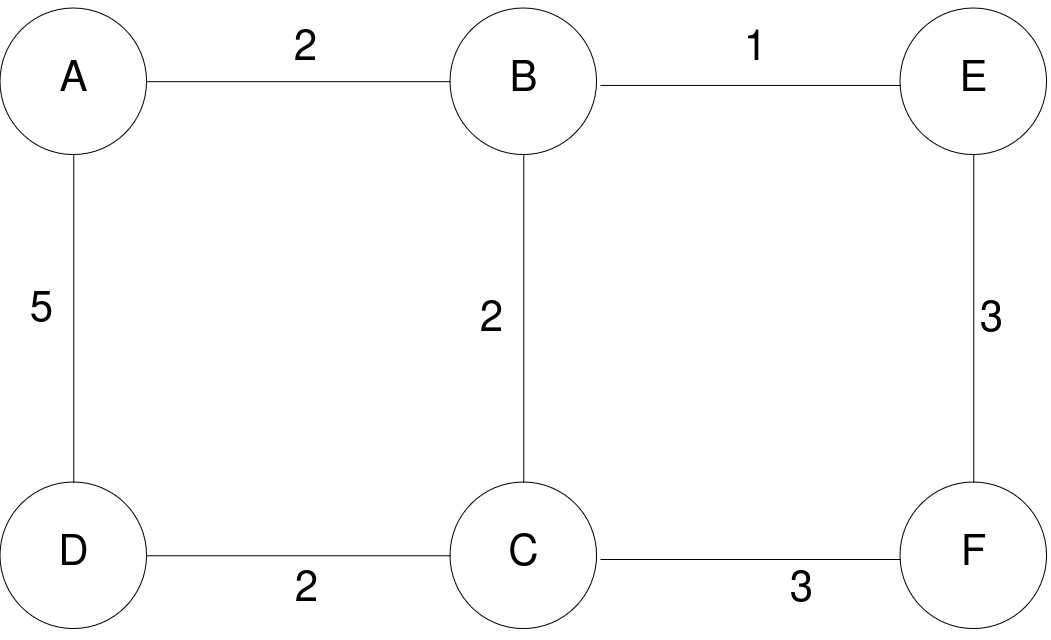
\includegraphics[width=0.6\textwidth]{figs/graph}
%    \end{center}
%
%    \subsection{Solution}
%
%
%    \begin{table}[H]
%        \begin{adjustbox}{center}
%            \begin{tabular}{|c|C{0.7cm}|C{0.7cm}||C{0.7cm}|C{0.7cm}||C{0.7cm}|C{0.7cm}||C{0.7cm}|C{0.7cm}||C{0.7cm}|C{0.7cm}||C{0.7cm}|C{0.7cm}|}
%                \hline
%                & \multicolumn{12}{|c|}{Distances and neighbours to each node} \\ \cline{2-13}
%                Node & \multicolumn{2}{|c||}{A} & \multicolumn{2}{|c||}{B} & \multicolumn{2}{|c||}{C} & \multicolumn{2}{|c||}{D} & \multicolumn{2}{|c||}{E} & \multicolumn{2}{|c|}{F} \\ \cline{2-13}
%                & D & N & D & N & D & N & D & N & D & N & D & N &
%                \hline
%                A & 0 & -- & 2 & B & ? & -- & 5 & D & ? & -- & ? & -- &
%                B & 2 & A & 0 & -- & 2 & C & ? & -- & 1 & E & ? & -- &
%                C & ? & -- & 2 & B & 0 & -- & 2 & D & ? & -- & 3 & F &
%                D & 5 & A & ? & -- & 2 & C & 0 & -- & ? & -- & ? & -- &
%                E & ? & -- & 1 & B & ? & -- & ? & -- & 0 & -- & 3 & F &
%                F & ? & -- & ? & -- & 3 & C & ? & -- & 3 & E & 0 & -- &
%                \hline
%            \end{tabular}\label{tab:table-a}
%        \end{adjustbox}
%        \caption{Solution to point 1}
%    \end{table}
%
%
%    \begin{table}[H]
%        \begin{adjustbox}{center}
%            \begin{tabular}{|c|C{0.7cm}|C{0.7cm}||C{0.7cm}|C{0.7cm}||C{0.7cm}|C{0.7cm}||C{0.7cm}|C{0.7cm}||C{0.7cm}|C{0.7cm}||C{0.7cm}|C{0.7cm}|}
%                \hline
%                & \multicolumn{12}{|c|}{Distances and neighbours to each node} \\ \cline{2-13}
%                Node & \multicolumn{2}{|c||}{A} & \multicolumn{2}{|c||}{B} & \multicolumn{2}{|c||}{C} & \multicolumn{2}{|c||}{D} & \multicolumn{2}{|c||}{E} & \multicolumn{2}{|c|}{F} \\ \cline{2-13}
%                & D & N & D & N & D & N & D & N & D & N & D & N &
%                \hline
%                A & 0 & -- & 2 & B & 4 & B & 5 & D & 3 & B & 6 & E &
%                B & 2 & A & 0 & -- & 2 & C & 4 & C & 1 & E & 4 & E &
%                C & 4 & B & 2 & B & 0 & -- & 2 & D & 3 & B & 3 & F &
%                D & 5 & A & 4 & C & 2 & C & 0 & -- & ? & -- & 5 & C &
%                E & 3 & B & 1 & B & 3 & B & ? & -- & 0 & -- & 3 & F &
%                F & ? & -- & 4 & E & 3 & C & 5 & C & 3 & E & 0 & -- &
%                \hline
%            \end{tabular}\label{tab:table-b}
%        \end{adjustbox}
%        \caption{Solution to point 2}
%    \end{table}
%
%
%    \begin{table}[H]
%        \begin{adjustbox}{center}
%            \begin{tabular}{|c|C{0.7cm}|C{0.7cm}||C{0.7cm}|C{0.7cm}||C{0.7cm}|C{0.7cm}||C{0.7cm}|C{0.7cm}||C{0.7cm}|C{0.7cm}||C{0.7cm}|C{0.7cm}|}
%                \hline
%                & \multicolumn{12}{|c|}{Distances and neighbours to each node} \\ \cline{2-13}
%                Node & \multicolumn{2}{|c||}{A} & \multicolumn{2}{|c||}{B} & \multicolumn{2}{|c||}{C} & \multicolumn{2}{|c||}{D} & \multicolumn{2}{|c||}{E} & \multicolumn{2}{|c|}{F} \\ \cline{2-13}
%                & D & N & D & N & D & N & D & N & D & N & D & N &
%                \hline
%                A & 0 & -- & 2 & B & 4 & B & 5 & D & 3 & B & ? & -- &
%                B & 2 & A & 0 & -- & 2 & C & 4 & C & 1 & E & 4 & E &
%                C & 4 & B & 2 & B & 0 & -- & 2 & D & 3 & B & 3 & F &
%                D & 5 & A & 4 & C & 2 & C & 0 & -- & 5 & B & 5 & C &
%                E & 3 & B & 1 & B & 3 & B & 5 & C & 0 & -- & 3 & F &
%                F & 6 & B & 4 & E & 3 & C & 5 & C & 3 & E & 0 & -- &
%                \hline
%            \end{tabular}\label{tab:table-c}
%        \end{adjustbox}
%        \caption{Solution to point 3}
%    \end{table}



%    \newpage
%    \section{Task}\label{sec:task-3}
%    Suppose we have the forwarding tables shown in Table 5-2 for nodes A and F in a network where all
%    links have cost 1.
%    Give a diagram of the smallest network consistent with these tables.
%
%    \subsection{Solution}
%
%     \begin{center}
%        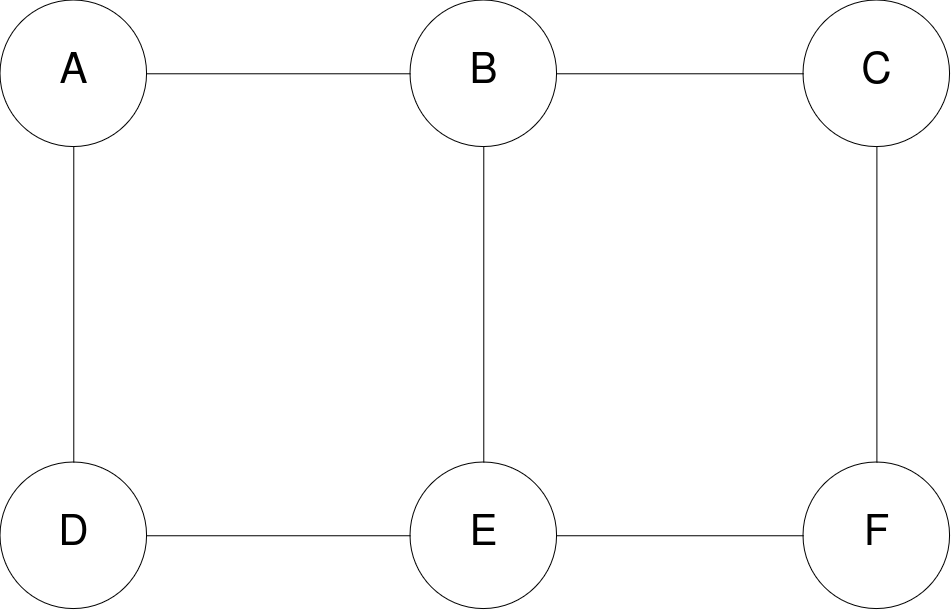
\includegraphics[width=0.6\textwidth]{figs/task3}
%    \end{center}
%     \newpage




    \setcounter{section}{3}

    \section{Task}
    An unfragmented IP packet, shown in Fig 5-2(a), has 1400 bytes of data and a 20-byte IP header.
    When the packet arrives at router RA, which has an MTU of 532 bytes, it has to be fragmented.
    The 3 fragmented packets are shown in Fig 5-2(b).
    Suppose these fragments all pass through another router RB with an MTU of 380 bytes, not counting the link header
    \begin{enumerate}
        \item Show the fragments the router RB produced.
        \item If the packet were originally fragmented for this MTU, how many fragments would be produced?
    \end{enumerate}

    \begin{center}
        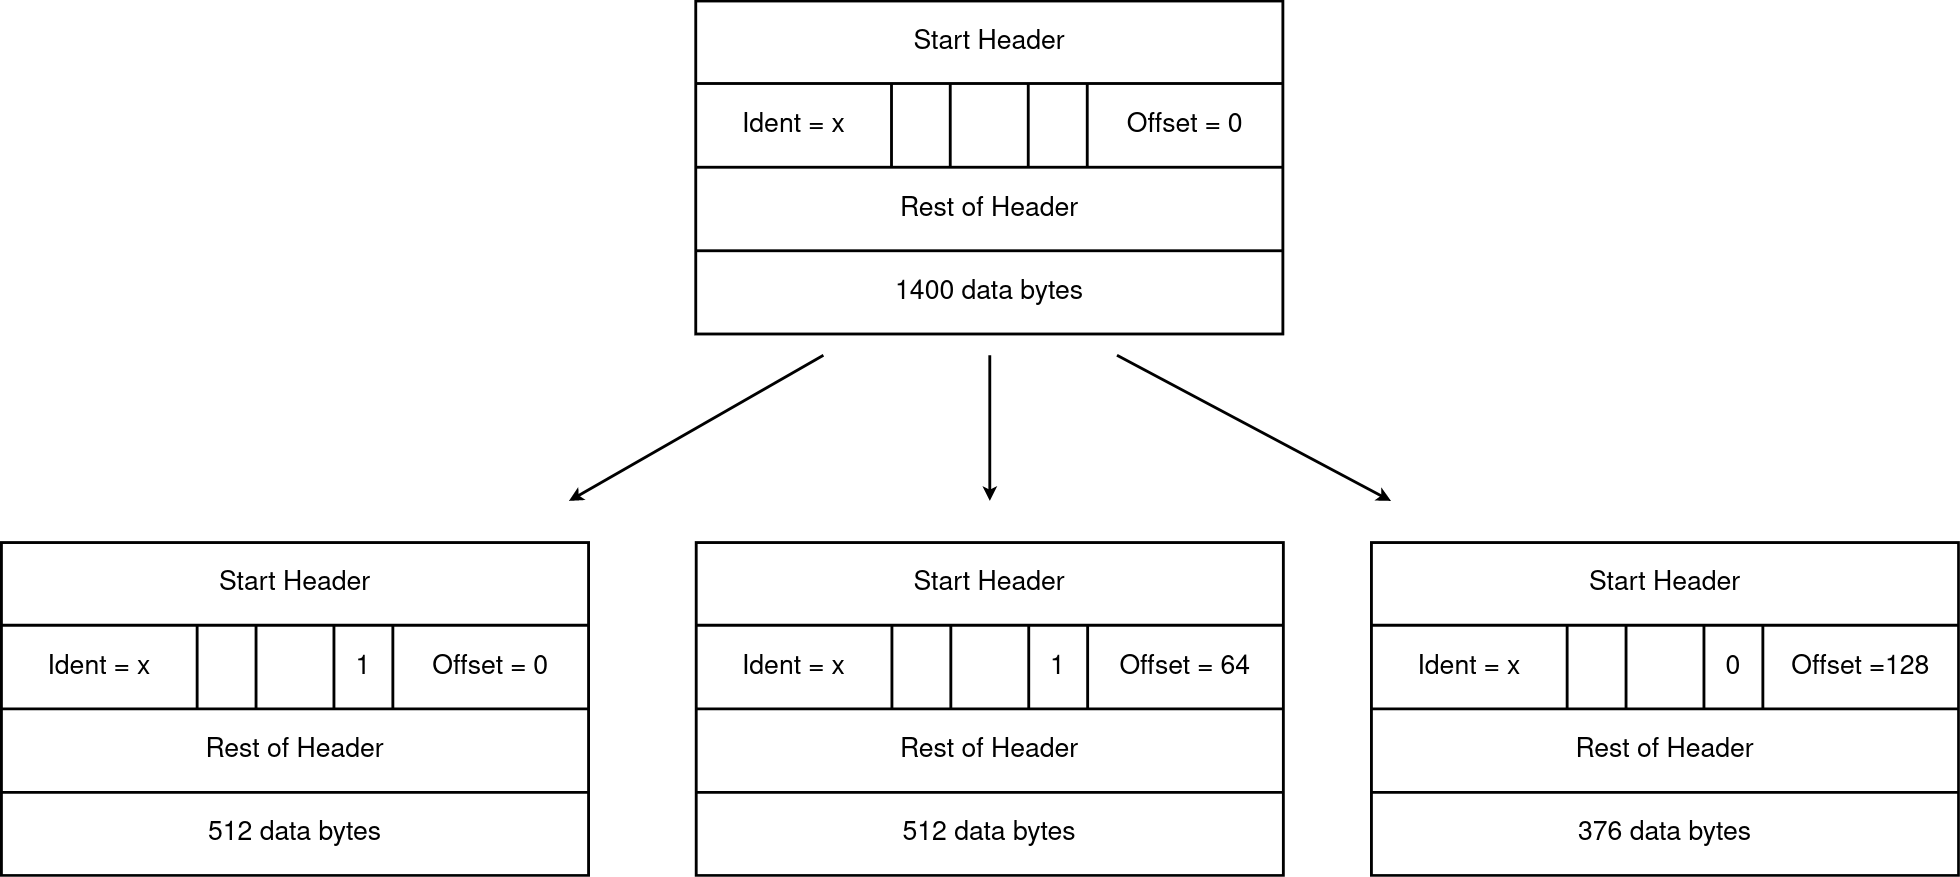
\includegraphics[width=1\textwidth]{figs/Task4}
    \end{center}

    \newpage
    \subsection{Solution}
    Internet protocol (IP) uses nontransparent fragmentation process to pass packets via routers.
    Hence, it treats each fragmented packet as original packet and does not reassemble fragments at intermediate routers.
    \paragraph{1.} After router RB receives first and second fragmented packets, it treats them separately and
    divides each of them to two smaller packets.
    Third packet is less than MTU of RB. Therefore, it is transmitted the same as it was.
    In total, router RB transmits 5 packets.

    \begin{center}
        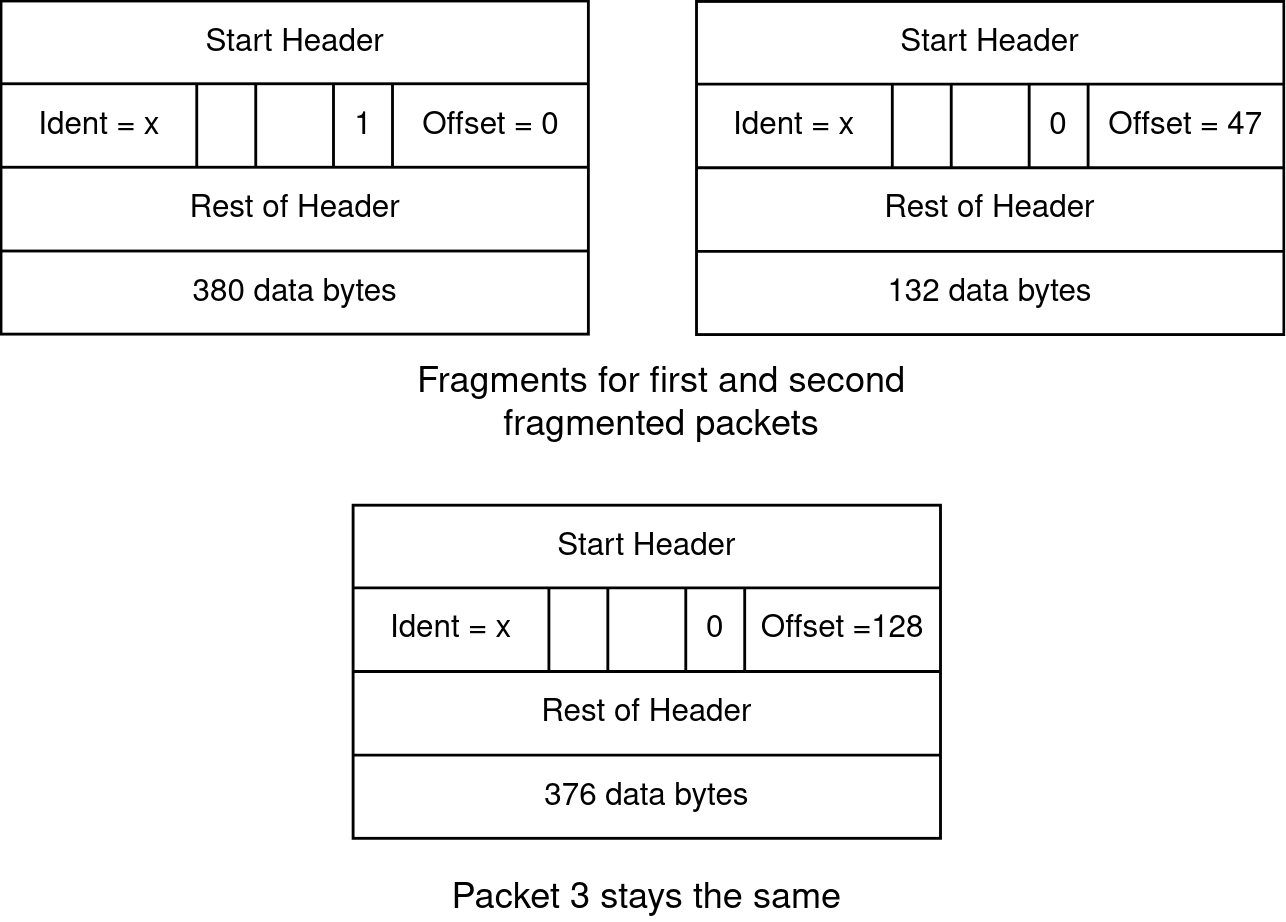
\includegraphics[width=0.75\textwidth]{figs/Sol4-1}
    \end{center}

    \paragraph{2.}
    The initial packet size is 1400 bytes.
    Thus, if it was directly send to router RB, the number of packets would be:
    $1400/380 \approx 3.6 = 4$ packets.



\end{document}